\section{Serial and parallel algorithms performance} \label{s:results:performance-serial-parallel}
	Performance of the parallel algorithms can be measured using different definitions and laws. Figures \ref{fig:speedup:crank-nicolson}, \ref{fig:speedup:explicit-upwind} and \ref{fig:speedup:implcit-upwind} show the \gls{speed-up} of parallel algorithms for problem of $10000$ and $1000$ grid points. In overall the lowest \gls{speed-up} is observed for Crank--Nicolson scheme -- nearly $1.1$ for $3$ processors for problem of $10000$ points. In case of $1000$ points it was impossible to get gain additional processors. Every new processor successively prolonged execution time, which can be observed in Figure \ref{fig:speedup:crank-nicolson}. The result is expected because according to \ref{fig:visualization:crank-nicolson} and \gls{computation-to-communication-ratio} only small part of scheme was be parallelized. Even if communication cost was optimized by spreading the grid to processor, the overall impact of quasi--serial part of numerical scheme has huge impact on performance and \gls{speed-up}.
	\begin{figure}[!htbp]
		\centering
		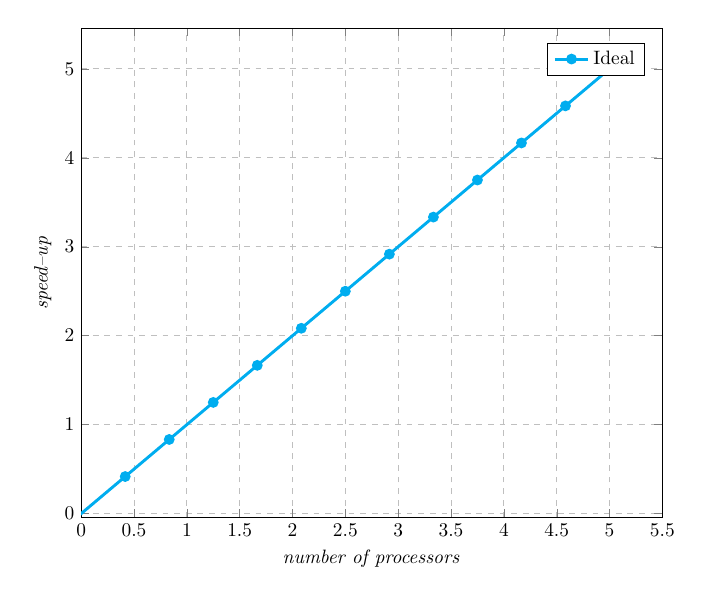
\begin{tikzpicture}[scale=0.7]	 	
		\pgfplotsset{width=\textwidth}
			\begin{axis}[
				xlabel = {\emph{number of processors}},
				ylabel = {\emph{speed--up}},
				%ymin = -1, ymax = 1,
				xmin = 0,% xmax = 13,
				%minor y tick num = 1,
				ymajorgrids=true,
				xmajorgrids=true,
				grid style=dashed,
				legend pos=north east
				]
				\addplot[mark=*, cyan, line width = 1.5pt] {x};
				\addlegendentryexpanded{Ideal};
				\addcustomplot{others/performance/crank-nicolson-parallel-final.csv}{red}{2}{10000 points}
				\addcustomplot{others/performance/crank-nicolson-parallel-final-1000.csv}{orange}{2}{1000 points}
			\end{axis}
		\end{tikzpicture}
		\caption{Speed-up of Crank-Nicolson numerical method.}
		\label{fig:speedup:crank-nicolson}
	\end{figure}
	The trend of \gls{speed-up}s shown in Figure \ref{fig:speedup:explicit-upwind} for $1000$ and $10000$ points is similar. Observation was made that for $1000$ points the maximum value is $1.65$ for $7$ processors. Problem of $10000$ gives \gls{speed-up} of $5.56$ for $32$ processors. According to Figure \ref{fig:visualization:explicit-upwind} we can observe that all the processors work simultaneously, which translates into overlap of the curves for small amount of processors for both sizes of problem.
	\begin{figure}[!htbp]
		\centering
		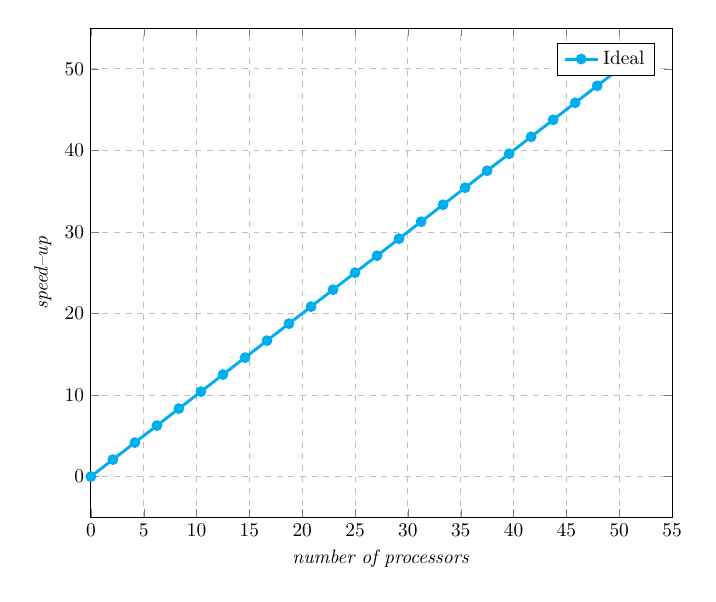
\begin{tikzpicture}[scale=0.7]	 	
			\pgfplotsset{width=\textwidth}
			\begin{axis}[
				xlabel = {\emph{number of processors}},
				ylabel = {\emph{speed--up}},
				%ymin = -1, ymax = 1,
				xmin = 0, %xmax = 13,
				%minor y tick num = 1,
				ymajorgrids=true,
				xmajorgrids=true,
				grid style=dashed,
				legend pos=north east
				]
				\addplot[domain=0:50,mark=*, cyan, line width = 1.5pt] {x};
				\addlegendentryexpanded{Ideal};
				\addcustomplot{others/performance/explicit-upwind-parallel-final.csv}{red}{2}{10000 points}
				\addcustomplot{others/performance/explicit-upwind-parallel-final-1000.csv}{orange}{2}{1000 points}
			\end{axis}
		\end{tikzpicture}
		\caption{Speed-up of Explicit Upwind numerical method.}
		\label{fig:speedup:explicit-upwind}
	\end{figure}
	Similarly to explicit upwind scheme, the implicit upwind \gls{speed-up} is also close to ideal. The further analysis of Figure \ref{fig:visualization:implicit-upwind} leads to conclusion that for $1000$ points usage of more than $24$ processors gives negative results in terms of execution time. For $10000$ points the limit was not found even $64$ processors this execution time is $11$ times faster than for a serial code, while for $10$ time smaller problem \gls{speed-up} is $2$ times less.
	\begin{figure}[!htbp]
		\centering
		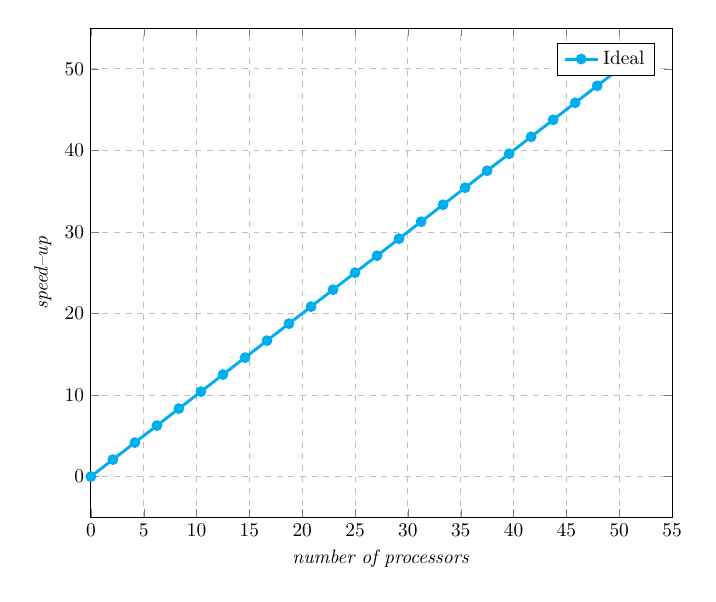
\begin{tikzpicture}[scale=0.7]	 	
		\pgfplotsset{width=\textwidth}
			\begin{axis}[
				xlabel = {\emph{number of processors}},
				ylabel = {\emph{speed--up}},
				%ymin = -1, ymax = 1,
				xmin = 0,% xmax = 13,
				%minor y tick num = 1,
				ymajorgrids=true,
				xmajorgrids=true,
				grid style=dashed,
				legend pos=north east
				]
				\addplot[domain=0:50, mark=*, cyan, line width = 1.5pt] {x};
				\addlegendentryexpanded{Ideal};
				\addcustomplot{others/performance/implicit-upwind-parallel-final.csv}{magenta}{2}{10000 points}
				\addcustomplot{others/performance/implicit-upwind-parallel-final-1000.csv}{green}{2}{1000 points}
			\end{axis}
		\end{tikzpicture}
		\caption{Speed-up of Implicit Upwind numerical method.}
		\label{fig:speedup:implcit-upwind}
	\end{figure}
	For all the schemes execution time decreased. The highest \gls{speed-up} observed for implicit upwind scheme. The worst result was given by Crank--Nicolson method giving nearly the same performance as the serial code. Communication cost for mentioned scheme is probably too high, which translates into performance. Summarizing obtained results improved performance, but none of scheme is even close to ideal.